\chapter{Multimodal Target Fusion and Entity-Level Registration}

\section{Introduction}
After the optical trajectory completion module in Chapter 3 has connected coordinate-missing optical observations to the existing trajectory system, the remaining challenge is to establish entity-level consistency across heterogeneous modalities. In the target fusion scenario considered in this thesis, optical, electromagnetic, SAR, and trajectory-based observations may all describe the same physical target, but they do so with different temporal sampling rates, localization accuracy, and attribute spaces. Therefore, even when each modality provides a completed trajectory, the identity relationship across modalities is still unknown.

This chapter addresses that problem through a trajectory-encoding and multi-set graph matching framework for cross-modal entity registration. The main idea is to treat each completed entity trajectory as a structured observation sequence, encode it into a compact embedding, and then perform joint registration across modality-specific entity sets instead of relying on isolated pairwise matching. Compared with direct one-to-one matching based only on local similarity, this design is more suitable for heterogeneous target fusion because it can simultaneously use temporal evolution, intra-set relational structure, and cross-set interaction. Related registration frameworks have shown similar value in robotics, remote sensing, multimodal model fusion, and medical-image analysis \cite{cattaneo2022lcdnet,maintz1998survey,zhou2025higoreg,chen2026multimodal,zhang2025optsar}.

Another important issue is that different modalities usually exhibit different observation quality. Optical trajectories may provide relatively intuitive spatial information but can be disturbed by occlusion and viewpoint changes. Electromagnetic observations may contain stable temporal signatures but weak spatial semantics. SAR observations often have sparse or structurally distorted target responses. For this reason, the proposed registration framework does not treat all cross-modal evidence equally. Instead, it introduces a reliability-aware fusion mechanism so that more reliable cross-set relations contribute more strongly to the final registration result.

The output of this chapter is a unified fused entity representation for each registered target. These fused entities preserve the trajectory information and modality-specific attributes collected across multiple sources, and they serve as the direct input to the behavior analysis tasks in Chapter 5. Accordingly, this chapter forms the methodological bridge between single-modal trajectory preparation and high-level group behavior understanding.

\section{Related Work}

\subsection{Single-Modal Trajectory Completion and Data Association}
Single-modal trajectory completion and data association are commonly formulated as the recovery of temporally coherent identities from fragmented observations. Early work treated this as a probabilistic association problem under clutter, missed detections, and local ambiguity, as represented by multiple-hypothesis and joint probabilistic data association frameworks \cite{reid1979mht,fortmann1983jpda}. Subsequent formulations introduced stronger global constraints by optimising association over graphs or network-flow structures, thereby improving long-range consistency under occlusion and fragmented detections \cite{schulter2017deepnetworkflow,dendorfer2021motchallenge}. In modern tracking-by-detection pipelines, the dominant strategy is to combine motion prediction with appearance or attribute embeddings, while more recent methods increasingly replace hand-crafted association rules with query propagation, memory, and end-to-end identity reasoning \cite{bewley2016sort,wojke2017deepsort,zhang2022bytetrack,aharon2022botsort,sun2021transtrack,meinhardt2022trackformer,zeng2022motr,gao2023memotr,gao2025motip}. Recent surveys describe this development as a shift from uncertainty-aware matching toward unified deep association models \cite{adzemovic2025motsurvey}. For the present thesis, however, the main role of these methods is upstream: they convert raw observations into temporally coherent entities within each modality. They do not by themselves resolve the central difficulty of multimodal fusion, namely how to establish correspondence between modality-specific entities when sampling density, localisation quality, and semantic representation differ across sensors.

\subsection{Multimodal Spatiotemporal Fusion}
Once single-modal completion has produced several modality-specific trajectory sets, multimodal spatiotemporal fusion aims to combine their complementary evidence into a more reliable target representation. Existing studies typically distinguish between feature-level fusion, which seeks a shared latent space for heterogeneous observations, decision-level fusion, which combines outputs from modality-specific predictors, and target-level fusion, which emphasises consistency of identity and trajectory across sources \cite{wu2024jointsemantic,chen2026multimodal,zhang2025optsar}. A common conclusion across these lines of work is that direct feature concatenation is rarely sufficient when modalities are asynchronous, noisy, or spatially misaligned. Effective fusion usually requires explicit treatment of temporal context, observation uncertainty, and inter-target structure. In the setting of this thesis, the inputs to fusion are no longer raw sensor measurements but completed modality-specific entities. The key issue therefore shifts from low-level feature combination to cross-modal correspondence establishment, because fusion quality is ultimately limited by whether the system can align the correct entities before aggregation.

\subsection{Graph Modeling and Graph Matching}
Graph-based modelling is attractive in trajectory analysis because identity is often supported not only by the attribute of one target, but also by its temporal continuity, neighbourhood configuration, and role within a local group. A graph representation can preserve these dependencies explicitly through node attributes and relation edges, and relation-aware graph reasoning has been shown to improve robustness when observations are incomplete or structurally ambiguous \cite{zhao2022graphreg,fu2023deepgraphmatching,liu2024s2anet}. Graph matching extends this idea from representation to correspondence: instead of matching isolated nodes independently, it searches for assignments that remain consistent with both local similarity and higher-order structure \cite{gold1996softassign,fu2023deepgraphmatching}. This is particularly relevant to heterogeneous target registration, where appearance may change substantially across modalities whereas aspects of the surrounding configuration may remain comparatively stable. For this reason, the present chapter adopts graph interaction and graph matching as the core route for cross-modal registration, so that modality-specific internal structure can be preserved while multiple entity sets are aligned jointly rather than by purely local comparisons.

\subsection{Entity-Level Target Registration and Alignment}
Entity-level target registration concerns whether observations or trajectories from different sources correspond to the same physical object. Compared with intra-modal association, this problem is harder because the entities to be aligned may differ simultaneously in feature space, localisation precision, temporal density, and noise characteristics. Existing work has approached this challenge through three broad lines. Classical geometric registration methods rely on rigid alignment and local correspondence consistency under relatively stable structure \cite{besl1992icp,rusinkiewicz2001icpvariants,chen1991rangeimages,segal2009gicp,tam2013registration}. Probabilistic and deformable formulations relax hard assignments and model uncertainty more explicitly, which improves robustness when overlap is partial or correspondence is ambiguous \cite{myronenko2010cpd,chui2003nonrigid}. More recent learning-based methods infer correspondences from learned descriptors or relation-aware features, while multi-set formulations attempt to reduce error accumulation by aligning several sets jointly rather than independently \cite{yew2020rpmnet,wang2019dcp,aoki2019pointnetlk,yanagi2025singleoptimization,maset2017multiview,torsello2011multiview,evangelidis2018joint,zhu2020multiviewem}. What remains less developed for the setting considered here is the case in which the registration units are not raw points but temporally aggregated entity trajectories with heterogeneous semantics across modalities. This gap motivates the strategy of this chapter, namely to encode trajectories into entity-level descriptors and then perform multi-set graph matching for cross-modal alignment.

\section{Trajectory Encoding for Entity Representation}

\subsection{Unified Representation of Completed Entity Trajectories}
Let \(m \in \mathcal{M}\) denote a sensing modality, where \(\mathcal{M}\) may include optical, electromagnetic, SAR, and other trajectory-producing sources. After single-modal completion, the \(m\)-th modality provides a set of completed entity trajectories
\begin{equation}
  \mathcal{T}^{(m)} = \{\tau_1^{(m)},\tau_2^{(m)},\ldots,\tau_{N_m}^{(m)}\},
\end{equation}
where \(N_m\) is the number of entities observed in modality \(m\). Each trajectory is organized as a time-ordered sequence of target states:
\begin{equation}
  \tau_i^{(m)} = \{x_{i,t_1}^{(m)},x_{i,t_2}^{(m)},\ldots,x_{i,t_{L_i}}^{(m)}\},
\end{equation}
where \(L_i\) is the trajectory length and \(x_{i,t}^{(m)}\) denotes the target state of entity \(i\) at time index \(t\).

To support subsequent cross-modal registration, all trajectories are converted into the same target-centered representation introduced in Chapter 2. For each state \(x_{i,t}^{(m)}\), this chapter writes
\begin{equation}
  x_{i,t}^{(m)} = \big[p_{i,t}^{(m)},\, v_{i,t}^{(m)},\, f_{i,t}^{(m)},\, c_{i,t}^{(m)},\, \mu_{i,t}^{(m)}\big],
\end{equation}
where \(p_{i,t}^{(m)}\) denotes spatial information, \(v_{i,t}^{(m)}\) denotes motion-related information, \(f_{i,t}^{(m)}\) denotes modality-specific attributes, \(c_{i,t}^{(m)}\) denotes confidence or observation quality, and \(\mu_{i,t}^{(m)}\in\{0,1\}\) denotes the validity mask. This representation is kept consistent with Eq.~\eqref{eq:chapter2-target-state}. In the subsequent encoding and fusion steps, invalid states are suppressed through the mask rather than treated as ordinary observations.

The detailed completion algorithm used to generate each \(\mathcal{T}^{(m)}\) is not the focus of this chapter. Instead, this chapter assumes that every modality has already produced a collection of reasonably complete trajectories and focuses on how these trajectory-level entities can be aligned across modalities. As illustrated in Fig.~\ref{fig:chapter4-trajectory-completion}, the single-modal completion stage is treated as a functional preparation step: missing or low-confidence segments are identified, spatio-temporal continuity constraints are used to recover a more continuous trajectory, and the resulting completed trajectory set is passed to the following graph matching stage.

\begin{figure}[htb]
  \centering
  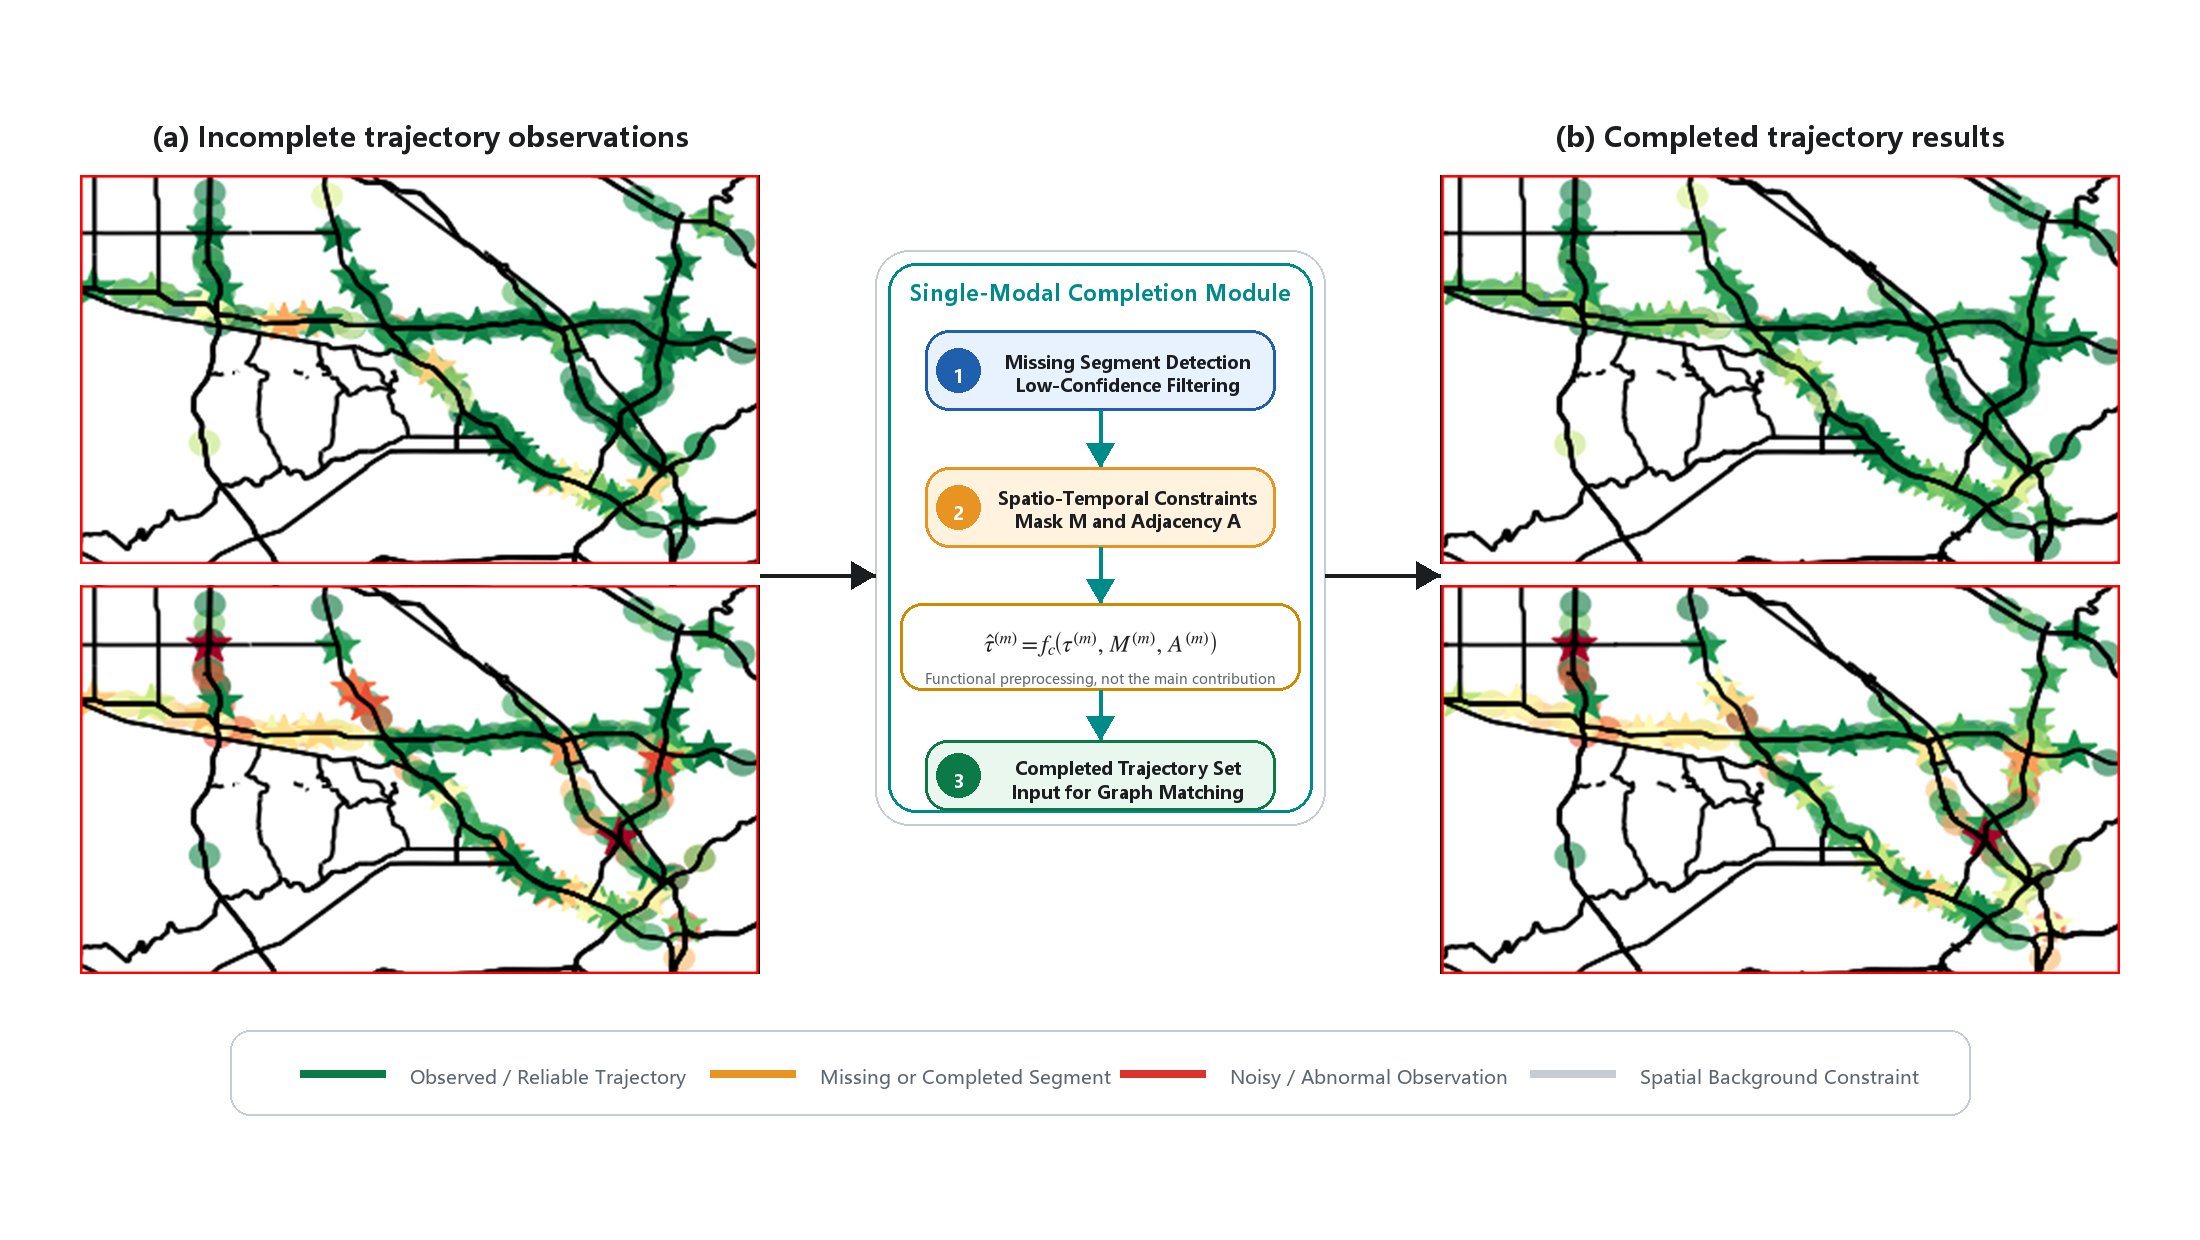
\includegraphics[width=\linewidth]{images/chapter4/trajectory_completion_original_based.png}
  \caption{Functional illustration of single-modal trajectory completion. Incomplete observations are organized through missing-segment detection and spatio-temporal continuity constraints, producing completed trajectory sets that serve as stable inputs for subsequent cross-modal graph matching.}
  \label{fig:chapter4-trajectory-completion}
\end{figure}

Therefore, the completed trajectory set serves as the direct input to the cross-modal registration framework. The notation below starts from \(\mathcal{T}^{(m)}\) and further encodes each completed trajectory into an entity-level descriptor for multi-set matching.

\subsection{Temporal Encoding of Entity Trajectories}
After the upstream completion stage has produced modality-specific entity trajectories, the next step is not to revisit the completion algorithms themselves, but to convert these trajectories into comparable units for cross-modal registration. Although the completed trajectories have a unified format, they still consist of variable-length state sequences. A direct comparison between raw sequences across modalities is inefficient and unstable, especially when the trajectories have different sampling intervals or different attribute dimensions. Therefore, the first task of this chapter is to encode each completed trajectory into a compact embedding that summarizes its temporal dynamics and target-level characteristics.

For each trajectory \(\tau_i^{(m)}\), a temporal encoder \(\Phi_{\mathrm{time}}(\cdot)\) is applied:
\begin{equation}
  h_i^{(m)} = \Phi_{\mathrm{time}}\big(\tau_i^{(m)}\big) \in \mathbb{R}^{d},
\end{equation}
where \(h_i^{(m)}\) is the \(d\)-dimensional entity embedding of the \(i\)-th trajectory in modality \(m\). The encoder may be implemented with a temporal aggregation network, a sequence encoder, or another trajectory modelling backbone. In this thesis, the exact architecture is less important than the role of the encoder: it compresses temporal evolution into a fixed-dimensional representation that can be compared and refined in the later graph matching stage. This step plays a role similar to the feature extraction stage used in feature-based registration pipelines such as PointNet, PointNetLK, DCP, and RPM-Net \cite{qi2017pointnet,aoki2019pointnetlk,wang2019dcp,yew2020rpmnet}.

The temporal embedding is expected to preserve three kinds of information. First, it should encode the motion evolution of the entity, including direction changes, velocity patterns, and temporal continuity. Second, it should retain modality-specific target attributes that remain informative after temporal aggregation. Third, it should be robust to local perturbations, missing states, and moderate observation uncertainty. In this way, the output embedding becomes a stable target-level descriptor rather than a simple average of per-time-step features.

After temporal encoding, each modality-specific entity set can be written as
\begin{equation}
  \mathcal{H}^{(m)} = \{h_1^{(m)},h_2^{(m)},\ldots,h_{N_m}^{(m)}\}.
\end{equation}
These embeddings form the basic node features used in the multi-set graph matching framework. Therefore, the function of Section 4.3 is simply to transform completed trajectories into compact entity representations, which are then refined and aligned in the next section.

\section{Cross-Modal Entity Registration Based on Multi-Set Graph Matching}

\subsection{Problem Formulation of Cross-Modal Entity Registration}
Given one reference modality and multiple source modalities, the goal of cross-modal entity registration is to determine which entities correspond to the same physical target across heterogeneous entity sets. Let the reference entity set be denoted by
\begin{equation}
  \mathcal{R} = \{r_1,r_2,\ldots,r_M\},
\end{equation}
and let the source entity sets be denoted by
\begin{equation}
  \mathcal{S} = \{\mathcal{S}_1,\mathcal{S}_2,\ldots,\mathcal{S}_K\}, \qquad
  \mathcal{S}_k = \{s^k_1,s^k_2,\ldots,s^k_{N_k}\},
\end{equation}
where each \(r_j\) or \(s^k_i\) is represented by the trajectory embedding obtained in Section 4.3.

The registration task is not to estimate a rigid geometric transformation as in classical point-set registration. Instead, it is to infer an entity-level correspondence structure between the source sets and the reference set. Formally, for each source set \(\mathcal{S}_k\), the objective is to estimate a correspondence matrix
\begin{equation}
  \Pi_k \in [0,1]^{N_k \times M},
\end{equation}
where \(\Pi_k(i,j)\) indicates the confidence that source entity \(s^k_i\) and reference entity \(r_j\) belong to the same physical target.

Unlike independent pairwise registration, the present formulation jointly uses all source sets during matching. This is important because different source modalities may provide complementary evidence. One source may preserve clearer temporal regularity, another may preserve more stable spatial structure, and a third may contribute stronger target-level semantics. A multi-set formulation makes it possible to use these complementary cues together instead of aligning every source in isolation.

Therefore, the cross-modal registration problem in this chapter can be summarized as follows: given multiple modality-specific entity sets represented by trajectory embeddings, construct a relational matching framework that refines node features through intra-set and cross-set interaction, evaluates the reliability of cross-modal evidence, and outputs a soft correspondence structure for entity-level alignment.

\begin{figure}[htb]
  \centering
  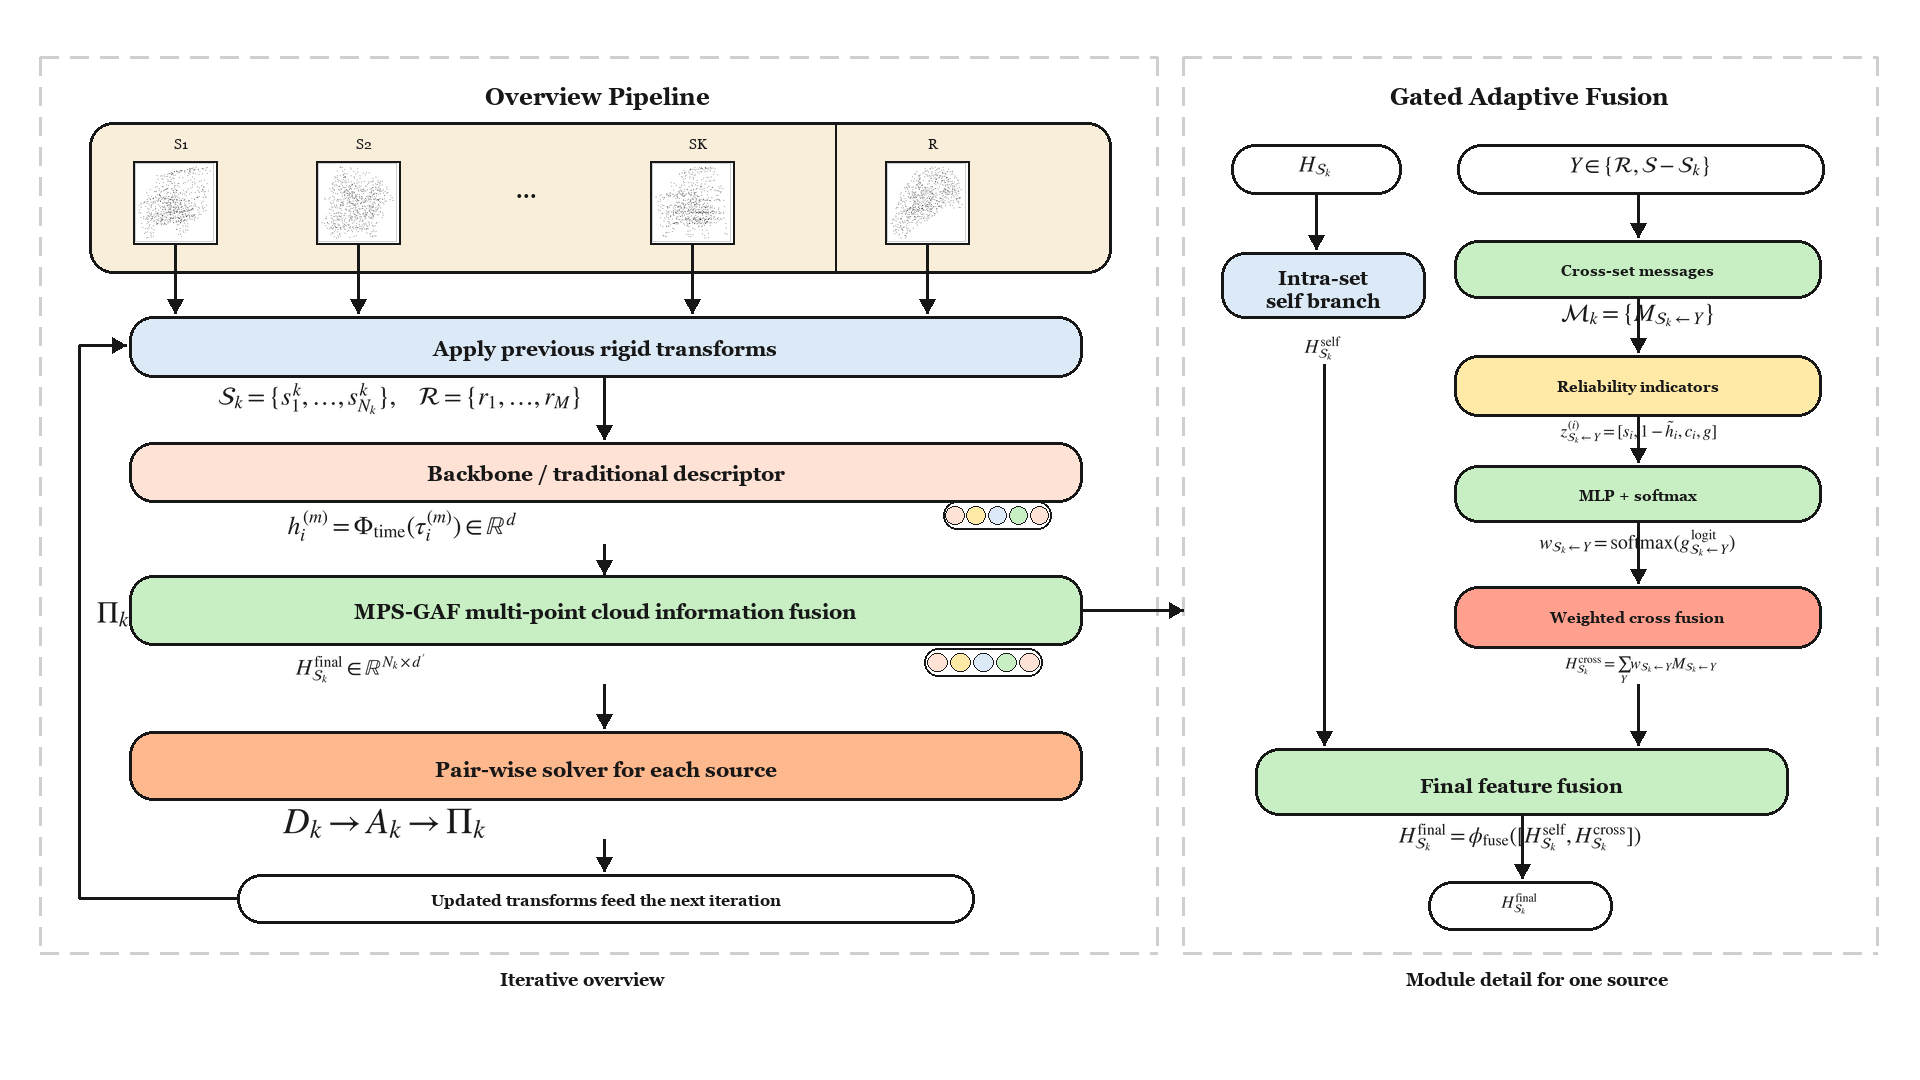
\includegraphics[width=\linewidth]{images/chapter4/multiset_graph_matching_framework.png}
  \caption{Overview of the multi-set graph matching framework. Completed entity trajectories are first encoded into target-level embeddings, then refined through intra-set interaction, cross-set information exchange, and reliability-aware fusion, and finally used to generate soft entity correspondences across modality-specific sets.}
  \label{fig:chapter4-framework}
\end{figure}

\subsection{Intra-Set and Cross-Set Feature Interaction}
The trajectory embeddings obtained in Section 4.3 provide compact target-level descriptors, but they do not yet fully encode the relational structure within each modality or the complementary interaction across modalities. To address this limitation, the proposed framework refines these embeddings in two stages: intra-set structural interaction and cross-set information exchange. The overall design follows the general idea of combining learned descriptors with relation-aware matching rather than relying only on isolated local similarity \cite{yew2020rpmnet,fu2023deepgraphmatching}.

For any entity set \(\mathcal{U}=\{u_1,\ldots,u_n\}\), where each \(u_i \in \mathbb{R}^{d}\), the framework first performs intra-set interaction to preserve modality-internal relational structure. The entity embeddings are projected into a latent interaction space:
\begin{equation}
  T_{\mathcal{U}} = U W_T,
\end{equation}
where \(U \in \mathbb{R}^{n \times d}\) is the stacked embedding matrix and \(W_T \in \mathbb{R}^{d \times d'}\) is a learnable projection. The pairwise similarity matrix inside the set is then computed as
\begin{equation}
  S^{\mathrm{intra}}_{\mathcal{U}} = T_{\mathcal{U}}T_{\mathcal{U}}^{\top}.
\end{equation}
After row-wise normalization, the resulting relation weights describe how strongly each entity should aggregate information from the other entities in the same set. This process helps the embedding of one entity absorb contextual information from neighboring entities and from the local group structure in the same modality.

The intra-set refined feature can therefore be written as
\begin{equation}
  H^{\mathrm{self}}_{\mathcal{U}} =
  \operatorname{softmax}\!\left(\frac{S^{\mathrm{intra}}_{\mathcal{U}}}{\tau}\right) U W_A + U W_S,
\end{equation}
where \(W_A\) and \(W_S\) are learnable mappings and \(\tau\) is a temperature parameter. The first term propagates structural information across related entities, while the second term preserves the original target identity branch.

After intra-set refinement, the framework performs cross-set interaction between different modality-specific entity sets. Let \(\mathcal{X}\) and \(\mathcal{Y}\) denote two distinct entity sets. Their embeddings are projected into a shared latent space:
\begin{equation}
  T^{\mathrm{cross}}_X = XW_X, \qquad T^{\mathrm{cross}}_Y = YW_Y,
\end{equation}
where \(X\) and \(Y\) are the stacked entity embedding matrices. The cross-set similarity matrix is then defined as
\begin{equation}
  S_{X \leftarrow Y}^{\mathrm{cross}} = T^{\mathrm{cross}}_X \big(T^{\mathrm{cross}}_Y\big)^\top.
\end{equation}
After normalization, the matrix gives the relevance of every entity in \(\mathcal{X}\) to all entities in \(\mathcal{Y}\). Based on this relation, a message from \(\mathcal{Y}\) to \(\mathcal{X}\) is aggregated:
\begin{equation}
  M_{X \leftarrow Y} =
  \operatorname{softmax}\!\left(\frac{S_{X \leftarrow Y}^{\mathrm{cross}}}{\tau}\right) YW_C.
\end{equation}

This design allows each entity set to receive complementary evidence from the reference set and from other source sets. In the present cross-modal scenario, such interaction is useful because one modality may compensate for another when local target evidence is weak, spatial precision is unstable, or a subset of entities is incompletely observed. Therefore, the role of this subsection is to refine the trajectory embeddings into relation-aware entity features before reliability-aware fusion is applied.

\subsection{Reliability-Aware Gated Fusion for Cross-Modal Matching}
If the messages collected from different entity sets are directly averaged, noisy or low-quality modality evidence may be propagated to the entire registration process. This problem is particularly serious in the present thesis setting because the sensing modalities do not have identical reliability. Their localization precision, observation density, and feature discriminability may vary significantly across scenes. Therefore, the cross-set messages should be fused adaptively rather than treated equally.

For a source entity set \(\mathcal{S}_k\), suppose that the framework has collected a group of incoming cross-set messages
\begin{equation}
  \mathcal{M}_k = \{M_{\mathcal{S}_k \leftarrow Y} \mid Y \in \{\mathcal{R}, \mathcal{S}\setminus \mathcal{S}_k\}\}.
\end{equation}
The objective of gated fusion is to determine how much information should be accepted from each incoming set \(Y\). To do this, the framework computes a group of reliability indicators from the cross-set similarity or correspondence distributions.

The first indicator is matching sharpness, which measures whether the relation distribution is concentrated around a few candidate correspondences. The second indicator is entropy, which measures uncertainty in the matching distribution. The third indicator is bidirectional consistency, which measures whether the relation from set \(X\) to set \(Y\) is supported by the reverse relation from \(Y\) back to \(X\). The fourth indicator is a global similarity measure between the two sets, which reflects their coarse semantic compatibility. Together, these indicators describe whether the message from \(Y\) should be trusted when refining the source set \(\mathcal{S}_k\).

More specifically, for the relation matrix \(E_{X \leftarrow Y}\), the sharpness of the \(i\)-th source entity is defined as
\begin{equation}
  s_i = \max_j E_{X \leftarrow Y}(i,j),
\end{equation}
the entropy is defined as
\begin{equation}
  \tilde{h}_i
  =
  - \frac{1}{\log |Y|}
  \sum_j E_{X \leftarrow Y}(i,j)\log E_{X \leftarrow Y}(i,j),
\end{equation}
and the bidirectional consistency is defined as
\begin{equation}
  c_i = \sum_j E_{X \leftarrow Y}(i,j) E_{Y \leftarrow X}(j,i).
\end{equation}
In addition, the global similarity score is written as
\begin{equation}
  g(X,Y) = \frac{\langle \bar{x},\bar{y} \rangle}{\|\bar{x}\|\,\|\bar{y}\|},
\end{equation}
where \(\bar{x}\) and \(\bar{y}\) denote the mean embeddings of the two sets. Since \(g(X,Y)\) is a set-level scalar while \(s_i\), \(\tilde{h}_i\), and \(c_i\) are entity-level indicators, the scalar value is broadcast to every entity in the source set before concatenation. These quantities allow the gate to jointly consider local matching confidence and coarse set-level compatibility.

For every incoming set \(Y\), the reliability vector is written as
\begin{equation}
  z_{\mathcal{S}_k \leftarrow Y}^{(i)}
  =
  \operatorname{Concat}[s_i,\ 1-\tilde{h}_i,\ c_i,\ g(X,Y)],
\end{equation}
where \(s_i\) denotes sharpness, \(\tilde{h}_i\) denotes normalized entropy, \(c_i\) denotes bidirectional consistency, and \(g(X,Y)\) denotes global similarity. The reliability vector is fed to a lightweight gating function \(G(\cdot)\):
\begin{equation}
  g_{\mathcal{S}_k \leftarrow Y}^{\mathrm{logit}} = \frac{1}{|\mathcal{S}_k|}\sum_i G\big(z_{\mathcal{S}_k \leftarrow Y}^{(i)}\big).
\end{equation}
The normalized fusion weight is then obtained by competitive softmax:
\begin{equation}
  w_{\mathcal{S}_k \leftarrow Y}
  =
  \frac{
    \exp\big(g_{\mathcal{S}_k \leftarrow Y}^{\mathrm{logit}}\big)
  }{
    \sum_{Y'} \exp\big(g_{\mathcal{S}_k \leftarrow Y'}^{\mathrm{logit}}\big)
  }.
\end{equation}

Based on these weights, the final cross-set feature of \(\mathcal{S}_k\) is written as
\begin{equation}
  H^{\mathrm{cross}}_{\mathcal{S}_k}
  =
  \sum_Y
  w_{\mathcal{S}_k \leftarrow Y} M_{\mathcal{S}_k \leftarrow Y}.
\end{equation}
This design makes the matching framework reliability-aware in two senses. First, high-confidence correspondence patterns contribute more strongly to the final feature. Second, unreliable modality evidence is suppressed instead of being injected into the registration stage without control. This is especially important in multimodal target fusion because the framework must tolerate modality-dependent localization errors and partial observation defects.

Finally, the self feature and the cross-set feature are fused into the refined registration feature:
\begin{equation}
  H^{\mathrm{final}}_{\mathcal{S}_k}
  =
  \phi_{\mathrm{fuse}}
  \big(
    \operatorname{Concat}[H^{\mathrm{self}}_{\mathcal{S}_k},\, H^{\mathrm{cross}}_{\mathcal{S}_k}]
  \big),
\end{equation}
where \(\phi_{\mathrm{fuse}}(\cdot)\) is a lightweight fusion mapping. The same operation is applied to the reference set. The output features then serve as the direct input to soft correspondence estimation.

\subsection{Soft Correspondence and Entity-Level Registration Output}
After relation-aware feature refinement, entity-level correspondences are estimated through a soft assignment mechanism. For each source set \(\mathcal{S}_k\) and the reference set \(\mathcal{R}\), the pairwise feature distance matrix is first computed:
\begin{equation}
  D_k(i,j)
  =
  \left\lVert
    H^{\mathrm{final}}_{\mathcal{S}_k}(i,:)
    -
    H^{\mathrm{final}}_{\mathcal{R}}(j,:)
  \right\rVert_2^2 .
\end{equation}
The distance matrix is then converted into an affinity matrix
\begin{equation}
  A_k(i,j) = -\beta_k \big(D_k(i,j)-\alpha_k\big),
\end{equation}
where \(\beta_k\) and \(\alpha_k\) control the scale and offset of the matching affinity.

To avoid forcing every entity into a hard one-to-one decision too early, the framework uses soft assignment and obtains a correspondence matrix
\begin{equation}
  \Pi_k = \operatorname{Sinkhorn}\big(\exp(A_k)\big).
\end{equation}
Here, \(\Pi_k(i,j)\) can be interpreted as the confidence that source entity \(s^k_i\) corresponds to reference entity \(r_j\). The soft assignment is more suitable than immediate hard matching because cross-modal alignment may remain ambiguous when observations are partially missing, local structures are similar, or modality gaps are strong. This formulation is consistent with the differentiable correspondence estimation strategy adopted in robust point matching pipelines such as RPM-Net \cite{yew2020rpmnet}.

The entity-level registration result is then derived from the soft correspondence structure. For each source entity, let
\begin{equation}
  j_i^{\ast} = \arg\max_j \Pi_k(i,j), \qquad
  p_i^{\ast} = \max_j \Pi_k(i,j).
\end{equation}
If \(p_i^{\ast} \ge \eta_{\mathrm{match}}\), the source entity is assigned to the reference identity \(r_{j_i^{\ast}}\). Otherwise, it is treated as an unmatched target:
\begin{equation}
  \mathcal{U}_k = \{s_i^k \mid p_i^{\ast} < \eta_{\mathrm{match}}\}.
\end{equation}
The unmatched set \(\mathcal{U}_k\) collects new, temporarily missing, or low-confidence entities that should not be forced into the current fusion groups. In this way, the output of registration is not limited to a closed-set one-to-one assignment, but remains compatible with realistic multimodal sensing conditions.

In implementation, the training objective of the registration stage follows the adopted underlying registration module rather than being redesigned independently in this chapter. More specifically, the entity-level formulation inherits the same correspondence-driven supervision and inlier regularization strategy used by the base matching framework \cite{wang2019dcp,yew2020rpmnet}. The emphasis of the present chapter is therefore on adapting the input representation, relation modeling, and output interpretation of the registration module to the multimodal entity-alignment setting.

Let \(\Gamma_k\) denote the final matched correspondence set between source set \(\mathcal{S}_k\) and reference set \(\mathcal{R}\). The registration output over all source modalities is written as
\begin{equation}
  \Gamma = \{\Gamma_1,\Gamma_2,\ldots,\Gamma_K\}, \qquad
  \Gamma_k = \{(s_i^k,r_{j_i^{\ast}})\mid p_i^{\ast}\ge \eta_{\mathrm{match}}\}.
\end{equation}
This output establishes the identity relationship required by multimodal target fusion, while \(\mathcal{U}_k\) preserves entities that should remain unmatched in the current step. Once the reliable entities have been aligned across modalities, the system can merge their trajectories and attributes into a unified target-level representation.

\section{Fusion Result Representation}

\subsection{Entity-Level Fusion Result Generation}
After the cross-modal correspondence structure \(\Gamma\) has been obtained, the next step is to convert registration results into entity-level fusion outputs. Let \(e_j\) denote the \(j\)-th fused entity in the unified representation space. All source entities that are assigned or strongly matched to the same reference identity are collected into one fusion group:
\begin{equation}
  \mathcal{C}_j = \{r_j\} \cup \{s^k_i \mid (s^k_i,r_j) \in \Gamma_k\}.
\end{equation}
For notational convenience, let the corresponding source-index set be
\begin{equation}
  \mathcal{I}_j = \{(k,i)\mid s_i^k \in \mathcal{C}_j\}.
\end{equation}

The trajectory information, modality-specific attributes, and correspondence confidence inside each group are then aggregated to generate the fused entity result. In generic form, the fused representation of entity \(e_j\) is written as
\begin{equation}
  e_j = \{T_j,\ F_j,\ C_j\},
\end{equation}
where \(T_j\) denotes the fused trajectory description, \(F_j\) denotes the fused multi-modal attribute representation, and \(C_j\) denotes confidence information derived from the registration stage.

For every member \(s_i^k \in \mathcal{C}_j\), let the registration-supported fusion score be
\begin{equation}
  \rho_{j}^{(k,i)} = \Pi_k(i,j)\,\bar{c}_i^{(k)},
\end{equation}
where \(\bar{c}_i^{(k)}\) denotes the average observation confidence of the \(i\)-th trajectory in modality \(k\). The normalized fusion weight is then written as
\begin{equation}
  \omega_{j}^{(k,i)} =
  \frac{\rho_{j}^{(k,i)}}{\sum_{(m,n)\in \mathcal{I}_j}\rho_{j}^{(m,n)}}.
\end{equation}
Based on these weights, the fused trajectory component at time index \(t\) is defined as
\begin{equation}
  T_j(t) =
  \frac{
    \sum_{(k,i)\in \mathcal{I}_j}
    \omega_{j}^{(k,i)} \mu_{i,t}^{(k)} p_{i,t}^{(k)}
  }{
    \sum_{(k,i)\in \mathcal{I}_j}
    \omega_{j}^{(k,i)} \mu_{i,t}^{(k)}
  },
\end{equation}
where \(\mu_{i,t}^{(k)}\in\{0,1\}\) is the validity mask defined in Chapter 2. In this way, missing observations do not force invalid trajectory values into the fused result.

The fused multi-modal attribute vector is obtained by weighted aggregation of modality-specific trajectory descriptors:
\begin{equation}
  F_j =
  \sum_{(k,i)\in \mathcal{I}_j}
  \omega_{j}^{(k,i)} \bar{f}_{i}^{(k)},
\end{equation}
where \(\bar{f}_{i}^{(k)}\) denotes the temporally aggregated attribute representation of the matched trajectory. Finally, the fusion confidence is computed as
\begin{equation}
  C_j =
  \sum_{(k,i)\in \mathcal{I}_j}
  \omega_{j}^{(k,i)} \rho_{j}^{(k,i)}.
\end{equation}
The quantity \(C_j\) jointly reflects matching confidence and trajectory quality, so that fused entities derived from weak correspondences or unreliable observations can be identified in later behavior analysis.

The trajectory component \(T_j\) therefore summarizes the motion of the entity after cross-modal alignment, while the feature component \(F_j\) preserves the modality-specific attributes contributed by optical, electromagnetic, SAR, and other sources. In practice, this means that the fused entity no longer belongs to one single modality, but becomes a target-centered object with cross-source information support.

Therefore, the registration stage and the fusion stage have different functions. Registration determines which entities correspond across modalities, while fusion determines how their information should be summarized into a single entity description. This distinction is important because the thesis does not equate correspondence estimation with full target fusion; instead, fusion is explicitly defined as a post-registration aggregation step.

\subsection{Unified Entity Representation for Behavior Analysis}
The final objective of this chapter is not merely to produce correspondence matrices, but to provide structured inputs for high-level behavior analysis. For that reason, the fused entity representation must remain interpretable and suitable for downstream temporal and group-level reasoning.

In this thesis, each fused entity is represented as a structured target record containing at least three categories of information: a trajectory component, a multi-modal attribute component, and a confidence component. The trajectory component supports later group motion analysis, spatiotemporal consistency modeling, and anomaly detection. The attribute component preserves complementary evidence that may help distinguish similar motion patterns under different sensing conditions. The confidence component records the reliability of the underlying cross-modal alignment and can later be used to control the influence of uncertain entities in behavior analysis.

Let the final fused entity set be denoted by
\begin{equation}
  \mathcal{F} = \{e_1,e_2,\ldots,e_{N_f}\},
\end{equation}
where \(N_f\) is the number of registered entities after cross-modal fusion. The set \(\mathcal{F}\) serves as the direct input to Chapter 5. In this way, the present chapter completes the transition from modality-specific trajectory sets to a unified entity space, which is the necessary basis for subsequent group behavior modeling and situation understanding.

\section{Experiments and Result Analysis}

\subsection{Experimental Setup and Evaluation Metrics}
The experiments in this chapter are designed to evaluate whether the proposed trajectory-encoding and multi-set graph matching framework can produce robust registration under both standard and degraded observation conditions. Since the core registration module is developed from an existing multi-set matching pipeline, the present experiments first validate its behavior in a controlled setting and then use the results to support its integration into the multimodal target fusion framework.

The experimental data are constructed on ModelNet40 \cite{wu2015shapenets}. Following the standard preprocessing protocol of the multi-set registration module, 2,048 points are uniformly sampled from each mesh and normalized to a unit sphere. During both training and testing, each example contains one target set and \(N\) source sets. Each source set is perturbed by a random rigid transformation, while the target set remains fixed. In the multi-set setting, the source sets are independently sampled for the same target object so that the registration method must jointly exploit complementary evidence across multiple views.

Although these experiments are performed on point-set data rather than directly on the multimodal target trajectories in the final system, they provide a controlled validation of the graph matching module used in this thesis. Their purpose is to verify whether the multi-set interaction and reliability-aware fusion design remain effective under clean, noisy, and incomplete conditions before the method is embedded into the entity-level registration stage of the target fusion framework.

The bridge between the benchmark setting and the thesis task lies in the matching mechanism rather than in the physical meaning of the raw data. In the benchmark experiments, each point set acts as a structured node set whose internal relations and cross-set correspondences must be inferred jointly. In the target-fusion system, the same role is played by modality-specific entity sets after temporal encoding, where each node corresponds to an entity trajectory or target state rather than a geometric point. Under this view, point-set correspondence matrices correspond to cross-modal entity association matrices, jitter and perturbation correspond to localization errors and attribute noise, and cropping or partial overlap correspond to missed detections, occlusion, and incomplete target observations. Therefore, the ModelNet40 experiments do not claim to reproduce the full multimodal fusion pipeline directly; instead, they provide controlled evidence that the underlying graph matching and reliability-aware registration mechanism is suitable for the entity-level alignment problem considered in this chapter.

Five metrics are used to evaluate registration quality, following \cite{yew2020rpmnet,wang2019dcp}. Two isotropic metrics are the Mean Isotropic Error of Rotation, denoted as \(\mathrm{MIE(R)}\), and the Mean Isotropic Error of Translation, denoted as \(\mathrm{MIE(t)}\). Two anisotropic metrics are the Mean Absolute Error of Rotation, denoted as \(\mathrm{MAE(R)}\), and the Mean Absolute Error of Translation, denoted as \(\mathrm{MAE(t)}\). In addition, the Corrected Chamfer Distance, denoted as \(\mathrm{CCD}\), measures the geometric discrepancy after registration while suppressing far outliers. In the present chapter, these metrics are used to evaluate the quality and robustness of the underlying registration module that supports cross-modal entity alignment.

The compared methods include classical registration baselines, deep pairwise registration methods, and representative multi-set registration methods, including ICP \cite{besl1992icp}, FGR \cite{zhou2016fgr}, MAC \cite{zhang2023mac}, PointNetLK \cite{aoki2019pointnetlk}, DCP \cite{wang2019dcp}, RPM-Net \cite{yew2020rpmnet}, JRMPC \cite{evangelidis2018joint}, and EMPMR \cite{zhu2020multiviewem}. In particular, the registration framework is implemented on top of RPM-Net \cite{yew2020rpmnet} so that the improvement introduced by multi-set interaction and gated fusion can be evaluated against a strong pairwise backbone. This comparison directly supports the main claim of this chapter: entity-level registration becomes more robust when multiple sets are jointly modeled instead of aligned independently. Additional dataset-wise benchmark results are reported in Appendix~\ref{chap:appendix-registration-benchmark}; they are kept outside the main chapter so that the main text can focus on the controlled ModelNet40 analysis.

\subsection{Performance Under Standard Conditions}
Under standard observation conditions, the purpose of the experiment is to examine whether the proposed framework can accurately align multiple source entity sets to the reference set when the observations are relatively complete and the noise level is moderate. In this setting, the main challenge is not severe corruption, but the need to exploit complementary cross-set information better than independent pairwise matching.

The expected behavior of the proposed framework is as follows. First, the temporal encoder provides compact entity embeddings that already preserve meaningful target evolution patterns. Second, intra-set interaction improves these embeddings by injecting structural context from the same modality. Third, cross-set interaction allows different source sets to exchange complementary evidence before correspondence estimation. As a result, the final soft correspondence matrices should be more stable and more discriminative than those obtained from direct pairwise matching.

Quantitatively, the results confirm this expectation. As shown in Table~\ref{tab:chapter4-clean}, the proposed multi-set graph matching framework achieves the best performance on all five metrics under clean conditions, with consistent improvements over the pairwise backbone RPM-Net. Although the gap is not large in this relatively easy setting, the result demonstrates that the explicit use of intra-set structure and cross-set complementarity can still reduce both rotation and translation errors.

\begin{table}[htb]
  \centering
  \caption{Performance under standard conditions. Bold and underline denote the best and second-best results.}
  \label{tab:chapter4-clean}
  \begin{tabular}{lccccc}
    \toprule
    Method & MIE(R) & MIE(t) & MAE(R) & MAE(t) & CCD \\
    \midrule
    ICP & 19.776 & 0.1370 & 11.710 & 0.0792 & 0.00358 \\
    FGR & 10.235 & 0.0603 & 6.506 & 0.0348 & 0.000869 \\
    MAC & 8.340 & 0.0539 & 6.774 & 0.0311 & 0.00110 \\
    PointNetLK & 8.842 & 0.0631 & 5.375 & 0.0323 & 0.00245 \\
    DCP & 6.733 & 0.0615 & 4.221 & 0.0313 & 0.00228 \\
    JRMPC & 3.578 & 0.0247 & 1.903 & 0.0142 & 0.00364 \\
    EMPMR & 20.141 & 0.1420 & 11.972 & 0.0819 & 0.00374 \\
    RPM-Net & \underline{0.468} & \underline{0.00347} & \underline{0.305} & \underline{0.00200} & \underline{0.0000496} \\
    RPM-Net + MPS-GAF & \textbf{0.465} & \textbf{0.00342} & \textbf{0.296} & \textbf{0.00198} & \textbf{0.0000485} \\
    \bottomrule
  \end{tabular}
\end{table}

The qualitative comparison in Fig.~\ref{fig:chapter4-clean} further shows that the jointly modeled source sets can be aligned more coherently to the target set. This observation is consistent with the role assigned to the method in this thesis: before the system aggregates information across modalities, it must first produce a stable correspondence structure, and the result under standard conditions verifies that the proposed framework is capable of doing so.

\begin{figure}[htb]
  \centering
  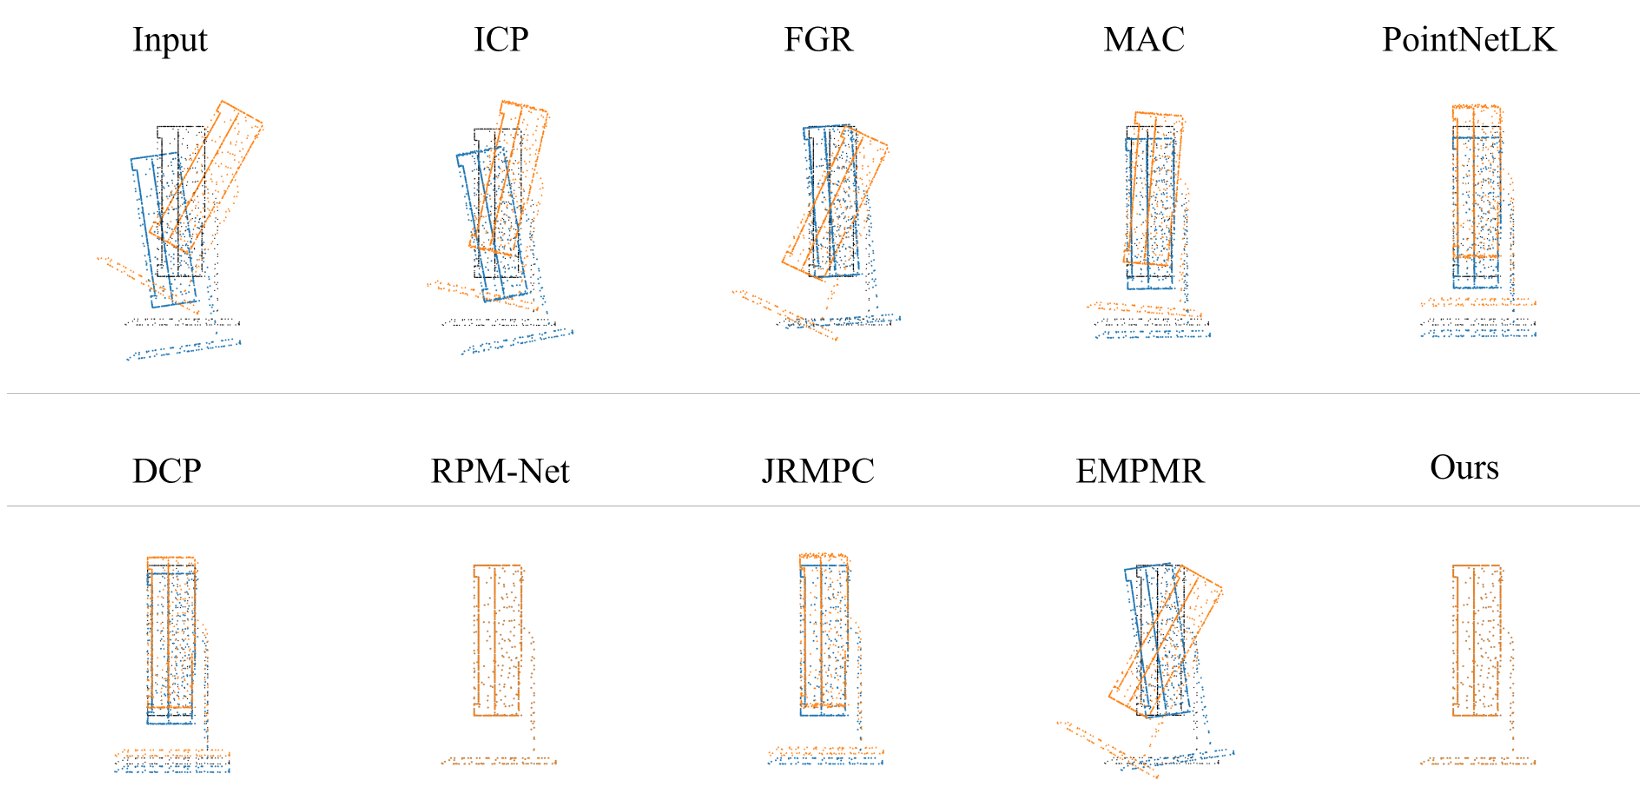
\includegraphics[width=\linewidth]{images/chapter4/registration_standard_conditions.png}
  \caption{Qualitative registration results under standard conditions. Black denotes the target set, while orange and blue denote two source sets.}
  \label{fig:chapter4-clean}
\end{figure}

\subsection{Performance Under Noisy or Incomplete Observations}
The more important test for multimodal target fusion lies in degraded conditions, where the observations are noisy, incomplete, or only partially available. This setting is closely related to real deployment because different sensing modalities rarely provide equally clean and complete target observations. In such cases, local entity descriptors may become ambiguous, and direct pairwise matching may be strongly affected by missing trajectories or unreliable spatial evidence.

The proposed framework addresses this difficulty in two ways. First, multi-set interaction allows one source set to benefit from complementary evidence in the others, reducing the risk that a single weak set dominates the registration result. Second, the reliability-aware gated fusion module explicitly down-weights low-confidence or conflicting incoming messages. Therefore, when observations are noisy or partially missing, the framework is expected to remain more stable than methods that simply average all cross-set information or match one source to the reference independently.

Under noisy conditions, random jitter is injected into both source sets and the target set. The quantitative results in Table~\ref{tab:chapter4-noise} show that the proposed framework still achieves the best performance on all five metrics. Relative to RPM-Net, the improvements are especially visible in the rotation and translation errors, indicating that the interaction modules and gated fusion improve stability under perturbation.

\begin{table}[htb]
  \centering
  \caption{Performance under noisy conditions. Bold and underline denote the best and second-best results.}
  \label{tab:chapter4-noise}
  \begin{tabular}{lccccc}
    \toprule
    Method & MIE(R) & MIE(t) & MAE(R) & MAE(t) & CCD \\
    \midrule
    ICP & 19.956 & 0.1360 & 11.772 & 0.0789 & 0.00320 \\
    FGR & 21.391 & 0.1630 & 13.076 & 0.0943 & 0.00771 \\
    MAC & 8.272 & 0.0572 & 6.234 & 0.0330 & 0.00123 \\
    PointNetLK & 8.842 & 0.0731 & 5.375 & 0.0423 & 0.00345 \\
    DCP & 8.733 & 0.0715 & 5.221 & 0.0413 & 0.00328 \\
    JRMPC & 3.761 & 0.0269 & 2.860 & 0.0155 & 0.00408 \\
    EMPMR & 20.219 & 0.1410 & 11.947 & 0.0817 & 0.00349 \\
    RPM-Net & \underline{1.955} & \underline{0.0137} & \underline{1.159} & \underline{0.00795} & \underline{0.000641} \\
    RPM-Net + MPS-GAF & \textbf{1.634} & \textbf{0.0128} & \textbf{1.016} & \textbf{0.00659} & \textbf{0.000624} \\
    \bottomrule
  \end{tabular}
\end{table}

The qualitative result in Fig.~\ref{fig:chapter4-noise} illustrates the same tendency. Even after perturbation, the multi-set framework produces a more coherent alignment than the pairwise strategy because it can integrate complementary evidence from multiple source sets rather than relying on one noisy matching path alone.

\begin{figure}[htb]
  \centering
  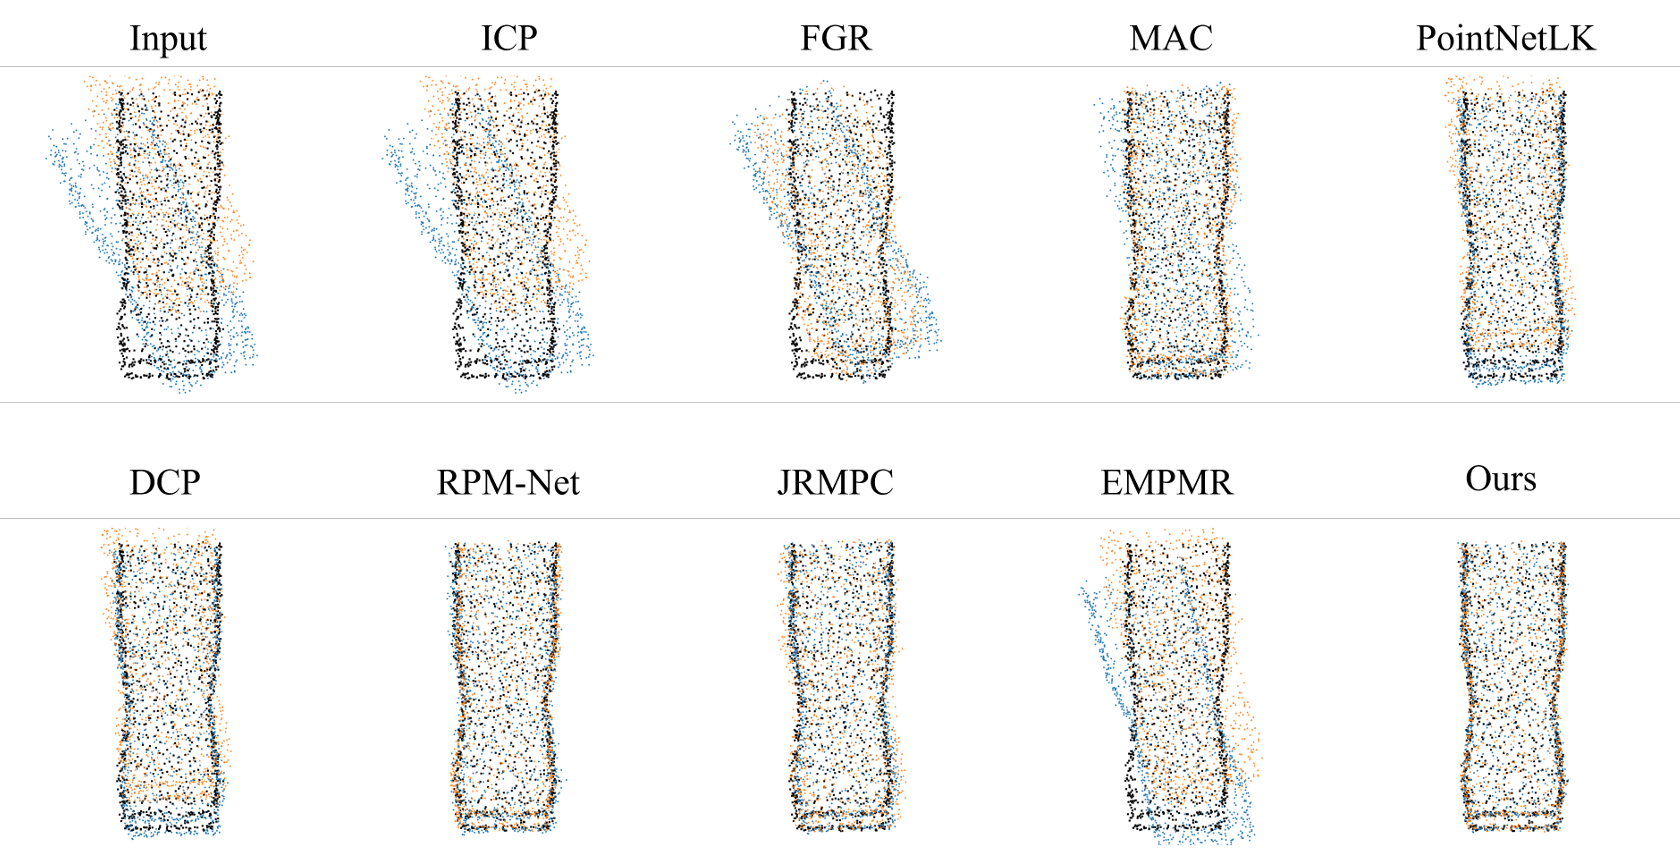
\includegraphics[width=\linewidth]{images/chapter4/registration_noisy_conditions.png}
  \caption{Qualitative registration results under noisy conditions. Black denotes the target set, while orange and blue denote two source sets.}
  \label{fig:chapter4-noise}
\end{figure}

The experiments further evaluate incomplete and partially observed conditions by cropping each set with a randomly oriented halfspace and combining the result with perturbation. This setting is especially relevant to the present thesis, because multimodal target observations are often spatially incomplete or only partially visible. As shown in Table~\ref{tab:chapter4-obstructed}, the proposed multi-set framework again outperforms all baselines under partial visibility.

\begin{table}[htb]
  \centering
  \caption{Performance under noisy and incomplete observations. Bold and underline denote the best and second-best results.}
  \label{tab:chapter4-obstructed}
  \begin{tabular}{lccccc}
    \toprule
    Method & MIE(R) & MIE(t) & MAE(R) & MAE(t) & CCD \\
    \midrule
    ICP & 38.195 & 0.3450 & 22.739 & 0.1990 & 0.0162 \\
    FGR & 48.141 & 0.3930 & 31.568 & 0.2270 & 0.0281 \\
    MAC & 9.409 & 0.0707 & 6.559 & 0.0408 & 0.0184 \\
    PointNetLK & 13.410 & 0.1650 & 8.803 & 0.0914 & 0.00817 \\
    DCP & 12.734 & 0.1500 & 8.094 & 0.0868 & 0.00773 \\
    JRMPC & 4.245 & 0.0418 & 2.363 & 0.0241 & 0.00503 \\
    EMPMR & 37.232 & 0.3370 & 22.058 & 0.1940 & 0.0153 \\
    RPM-Net & \underline{3.228} & \underline{0.0332} & \underline{2.137} & \underline{0.0193} & \underline{0.000852} \\
    RPM-Net + MPS-GAF & \textbf{2.956} & \textbf{0.0321} & \textbf{1.955} & \textbf{0.0172} & \textbf{0.000723} \\
    \bottomrule
  \end{tabular}
\end{table}

The qualitative case in Fig.~\ref{fig:chapter4-crop} shows why the gain is larger in this more difficult setting. The adaptive gate fusion mechanism suppresses inconsistent or weak source evidence and preserves cross-set support from the more reliable local structures. This characteristic is precisely the reason why the method is useful for multimodal target fusion, where incomplete observations are common.

\begin{figure}[htb]
  \centering
  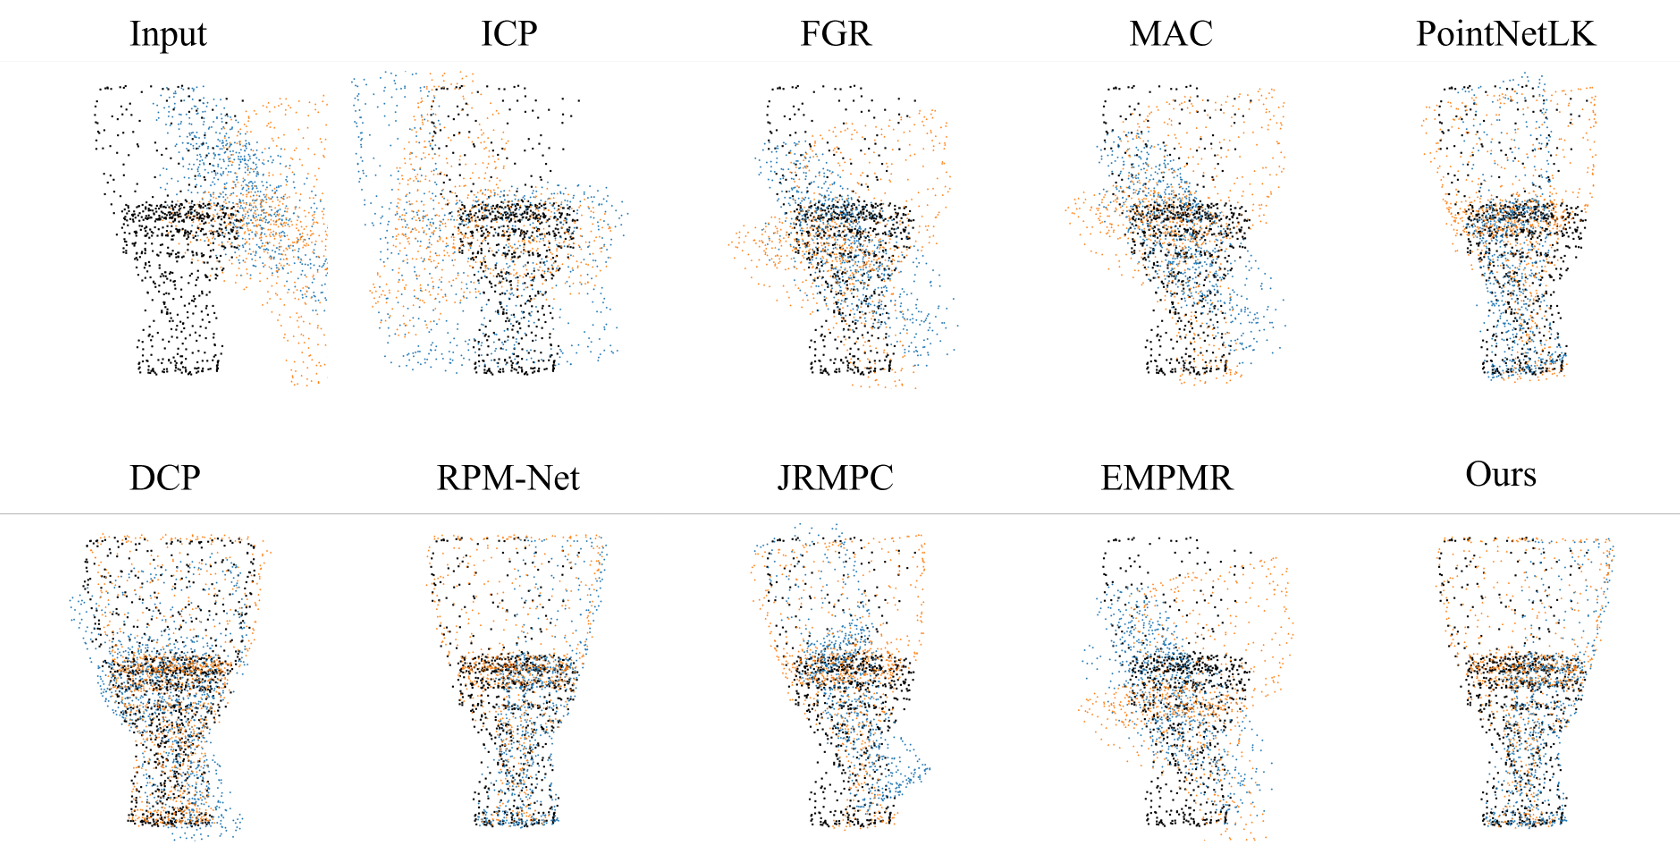
\includegraphics[width=\linewidth]{images/chapter4/registration_noisy_incomplete_conditions.png}
  \caption{Qualitative registration results under noisy and incomplete observations. Black denotes the target set, while orange and blue denote two source sets.}
  \label{fig:chapter4-crop}
\end{figure}

\subsection{Discussion of Cross-Modal Registration Results}
The experimental results should be interpreted from the perspective of the proposed registration mechanism rather than as isolated numerical gains. When the framework performs well, the improvement is mainly due to three factors. First, trajectory encoding converts variable-length entity observations into stable embeddings, making cross-modal comparison more feasible. Second, intra-set and cross-set interaction inject relation-aware context into the matching process, which reduces the ambiguity of local entity features. Third, reliability-aware fusion prevents low-quality source evidence from overwhelming the final registration decision.

From a multimodal target fusion viewpoint, the significance of these results is that entity registration becomes more robust when it is treated as a structured multi-set problem instead of a collection of independent pairwise tasks. This is consistent with the practical intuition that the same physical target should be supported by multiple forms of evidence across modalities, and that the registration framework should actively use this complementarity.

The first additional observation concerns the effect of increasing the number of source sets. As shown in Fig.~\ref{fig:chapter4-numsources}, the registration performance consistently improves when more source sets are introduced. This trend verifies the multi-set hypothesis of the present chapter: if the system can exploit complementary structure from multiple sources and selectively suppress unreliable evidence, then registration quality should improve as more informative sets become available.

This observation is also relevant to the implementation system described later. In the demonstration workflow, different sensing sources and different experimental outputs may not have identical quality, density, or temporal coverage. A registration module that can aggregate multiple source sets is therefore more suitable than a rigid pairwise matcher, because it can keep useful evidence while reducing the influence of incomplete observations. At the same time, the result should not be read as an unlimited scaling claim. Adding more sources is useful only when they provide complementary and reasonably reliable structure; otherwise, the reliability-aware fusion module is still needed to prevent noisy evidence from degrading the final correspondence.

\begin{figure}[H]
  \centering
  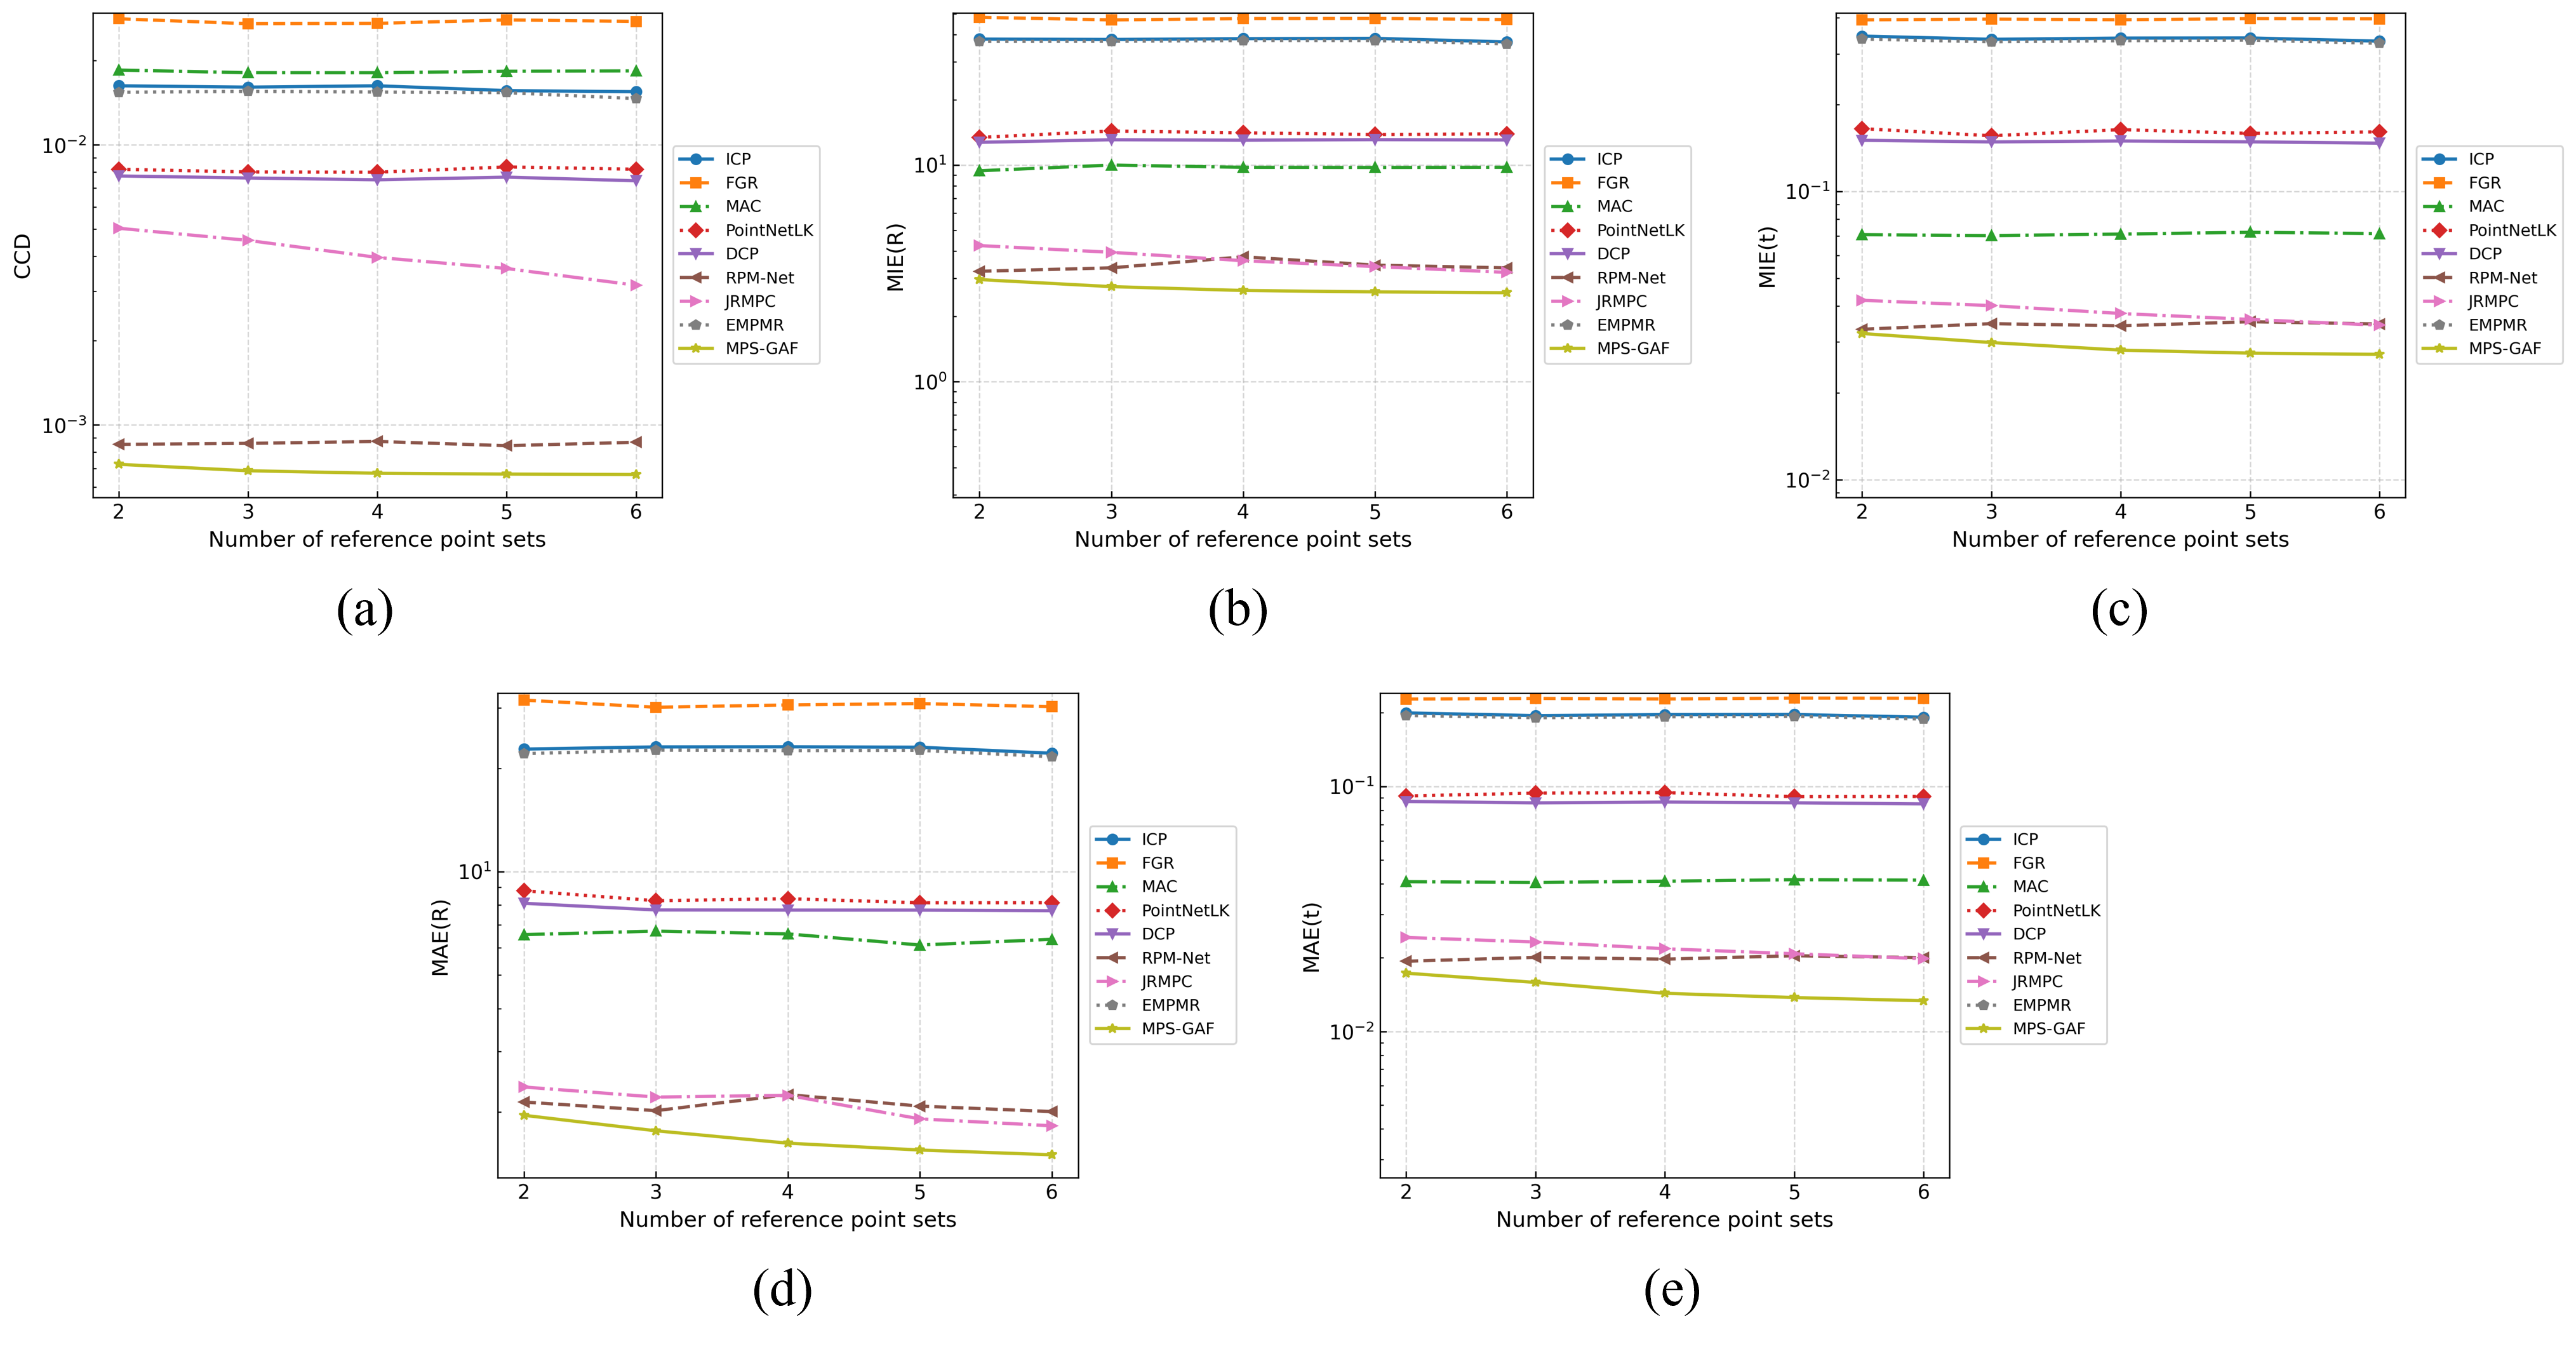
\includegraphics[width=\linewidth]{images/chapter4/registration_source_set_number.png}
  \caption{Registration performance across different numbers of source sets. The result shows that the multi-set interaction framework benefits from increasing source-set complementarity.}
  \label{fig:chapter4-numsources}
\end{figure}

The second observation concerns method generality. The results also show that the multi-set interaction module can improve several representative pairwise backbones. This is important for the present thesis because the cross-modal entity-registration stage should remain modular rather than tied to one single encoder or matcher. Table~\ref{tab:chapter4-backbone} and Fig.~\ref{fig:chapter4-backbone} summarize the evidence that the framework remains effective across multiple backbones under difficult conditions.

\begin{table}[H]
  \centering
  \caption{Performance gain across different backbone networks under difficult conditions.}
  \label{tab:chapter4-backbone}
  \begin{tabular}{lccccc}
    \toprule
    Method & MIE(R) & MIE(t) & MAE(R) & MAE(t) & CCD \\
    \midrule
    DCP & 34.431 & 0.478 & 20.450 & 0.275 & 0.0443 \\
    DCP + MPS-GAF & \textbf{29.074} & \textbf{0.397} & \textbf{16.824} & \textbf{0.229} & \textbf{0.0333} \\
    PointNetLK & 51.315 & 0.562 & 29.671 & 0.324 & 0.0681 \\
    PointNetLK + MPS-GAF & \textbf{45.828} & \textbf{0.535} & \textbf{26.493} & \textbf{0.309} & \textbf{0.0601} \\
    RPM-Net & 35.063 & 0.391 & 25.363 & 0.225 & 0.0113 \\
    RPM-Net + MPS-GAF & \textbf{30.124} & \textbf{0.343} & \textbf{22.531} & \textbf{0.202} & \textbf{0.0103} \\
    \bottomrule
  \end{tabular}
\end{table}

The table gives the quantitative evidence for the modularity of the framework. The following visual comparison complements this evidence by showing the same trend in registration quality under representative backbone choices.

\begin{figure}[htb]
  \centering
  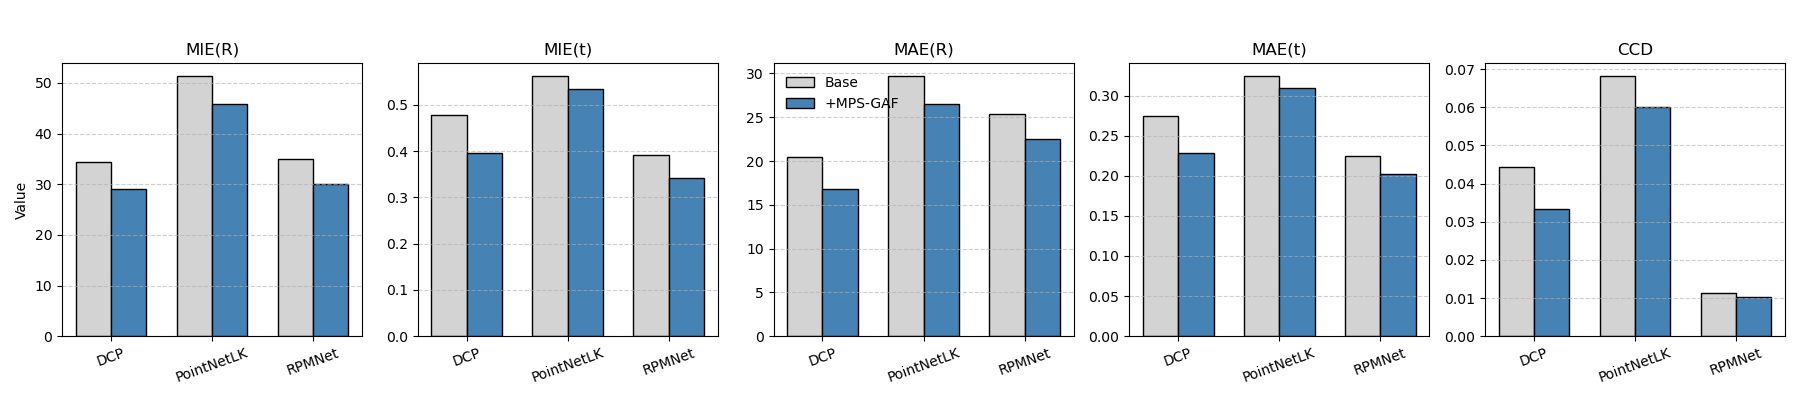
\includegraphics[width=0.9\linewidth]{images/chapter4/registration_backbone_comparison.png}
  \caption{Comparison of the multi-set graph matching framework across different backbones. The result shows that the reliability-aware multi-set interaction mechanism consistently improves several representative pairwise registration networks.}
  \label{fig:chapter4-backbone}
\end{figure}

At the same time, the experimental analysis also reveals the limitation of the present approach. If the trajectory embeddings are too weak, or if all source sets are simultaneously degraded, then even relation-aware matching may remain uncertain. In addition, the final fusion quality still depends on the quality of the completed trajectories supplied by the upstream modules. These limitations do not invalidate the present chapter, but they clarify the conditions under which multi-set registration is most effective and motivate later extensions that can further strengthen trajectory encoding and confidence modeling.

\section{Chapter Summary}
This chapter studies multimodal target fusion from the perspective of cross-modal entity registration. First, completed trajectories from different modalities are converted into a unified target-centered representation and encoded into compact trajectory embeddings. Second, a multi-set graph matching framework refines these embeddings through intra-set interaction and cross-set information exchange. Third, a reliability-aware gated fusion mechanism adaptively weights heterogeneous matching evidence and produces soft entity-level correspondences across modality-specific entity sets. Finally, the registered entities are merged into unified fused target representations, which serve as the input to the behavior analysis tasks in the next chapter.
